
\documentclass{article} % For LaTeX2e
\usepackage{iclr2027_conference,times}

% Optional math commands from https://github.com/goodfeli/dlbook_notation.
\input{math_commands.tex}

\usepackage{float}
\usepackage{longtable}
\usepackage{hyperref}
\hypersetup{hidelinks}
\usepackage{url}
\usepackage{xcolor}
\usepackage{xspace}
\usepackage{booktabs}
\usepackage{graphicx}
\usepackage{multirow}
\usepackage{makecell}


\title{APT-Bench: Supplementary Sampling Analyses}
% Global paper constants

\newcommand{\ourmethod}{Soft-cascade Transformer\xspace}

\newcommand{\numsubtypes}{27}

% Authors must not appear in the submitted version. They should be hidden
% as long as the \iclrfinalcopy macro remains commented out below.
% Non-anonymous submissions will be rejected without review.

\author{Antiquus S.~Hippocampus, Natalia Cerebro \& Amelie P. Amygdale \thanks{ Use footnote for providing further information
about author (webpage, alternative address)---\emph{not} for acknowledging
funding agencies.  Funding acknowledgements go at the end of the paper.} \\
Department of Computer Science\\
Cranberry-Lemon University\\
Pittsburgh, PA 15213, USA \\
\texttt{\{hippo,brain,jen\}@cs.cranberry-lemon.edu} \\
\And
Ji Q. Ren \& Yevgeny LeNet \\
Department of Computational Neuroscience \\
University of the Witwatersrand \\
Joburg, South Africa \\
\texttt{\{robot,net\}@wits.ac.za} \\
\AND
Coauthor \\
Affiliation \\
Address \\
\texttt{email}
}

% The \author macro works with any number of authors. There are two commands
% used to separate the names and addresses of multiple authors: \And and \AND.
%
% Using \And between authors leaves it to \LaTeX{} to determine where to break
% the lines. Using \AND forces a linebreak at that point. So, if \LaTeX{}
% puts 3 of 4 authors names on the first line, and the last on the second
% line, try using \AND instead of \And before the third author name.

\newcommand{\todo}[1]{\textcolor{red}{TODO: #1}}


\begin{document}
\maketitle
\begin{abstract}
This standalone report preserves the supporting subject--cell sampling
analyses previously included in the APT-Bench manuscript. These experiments
address allocation policies, training-label distribution, and uncertainty,
not the primary APT cell-typing benchmark or external disease validation.
The report retains the historical analyses and their limitations; separation
from the paper does not delete results or promote them to independent claims.
\end{abstract}
\section{Scope and Statistical Units}
The main APT-Bench paper evaluates APT-only cell typing on new patients.
This report instead compares training-allocation policies on APT, COMBAT,
and OneK1K. Subject-balanced pooled Macro-F1 normalizes each subject's
confusion matrix by its total cell count before pooling, using a fixed
class universe and zero contribution for undefined class F1. Cell-weighted
historical results are labeled separately. The report preserves fixed-cohort
and fixed-fold limitations, differentiates stability ranges from confidence
intervals for mean effects, and does not claim a universal scaling law.
\section{Synthetic Validation}
\subsection{Sequential Controls: Synthetic Mechanism Check}
\label{sec:appendix:sequential_simulation}

The real-data class-matched sampler fixes class quotas and spreads cells across
donors within each class. To distinguish these operations, we implement four
conditions with common random cell priorities and nested development subject
sets: (A) uniform pooled-cell sampling; (B) restriction to the eight-subject
reference class set, reserving one cell per class before uniform filling;
(C) exact reference class quotas with uniform within-class sampling; and
(D) the same quotas with capacity-constrained donor round robin in randomized
donor order. At fixed total, exact class proportions and exact counts are
equivalent constraints, not separate ablations. This A condition is not the
legacy equal-cell-per-subject sampler. Sequential contrasts are order-dependent
descriptions, not causal mediation estimates.

We evaluate this implementation on synthetic data, not a semi-synthetic clinical
cohort. Each of 20 seeds generates six class centers $\mu_k\sim
\mathcal{N}(0,s^2I_{12})$ and 48 subjects with 400 cells each. Subject label
probabilities are $\operatorname{softmax}(\eta_p)$, where
$\eta_p\sim\mathcal{N}(0,m^2I_6)$, and features are
$x_{pi}=\mu_{y_{pi}}+b_p+\epsilon_{pi}$, with
$b_p\sim\mathcal{N}(0,a^2I_{12})$ and
$\epsilon_{pi}\sim\mathcal{N}(0,I_{12})$ independently. We vary
$a,m\in\{0,1.5\}$ and $s\in\{0.5,1.5\}$. The first 32 subjects form the
development pool; the remaining 16 are untouched test subjects. An unweighted
LR probe is refit with training-only standardization for each condition and
$P\in\{8,32\}$ at total 1,600 training cells. All conditions reuse the same
realization and test subjects within a seed.

\begin{table}[htbp]
\centering\small
\begin{tabular}{rrrccc}
\toprule
Offset & Mixture & Separation & A: Unmatched & C: Quota & D: Quota + donor \\
\midrule
0.0 & 0.0 & 0.5 & \shortstack{+0.001\\{}[-0.007,+0.007]} & \shortstack{+0.001\\{}[-0.007,+0.008]} & \shortstack{+0.001\\{}[-0.006,+0.007]} \\
0.0 & 0.0 & 1.5 & \shortstack{-0.000\\{}[-0.003,+0.001]} & \shortstack{-0.000\\{}[-0.003,+0.002]} & \shortstack{-0.000\\{}[-0.003,+0.001]} \\
0.0 & 1.5 & 0.5 & \shortstack{+0.024\\{}[-0.005,+0.075]} & \shortstack{-0.001\\{}[-0.012,+0.010]} & \shortstack{-0.002\\{}[-0.012,+0.007]} \\
0.0 & 1.5 & 1.5 & \shortstack{+0.002\\{}[-0.005,+0.009]} & \shortstack{+0.000\\{}[-0.005,+0.003]} & \shortstack{-0.000\\{}[-0.003,+0.005]} \\
1.5 & 0.0 & 0.5 & \shortstack{+0.028\\{}[-0.028,+0.103]} & \shortstack{+0.028\\{}[-0.023,+0.103]} & \shortstack{+0.031\\{}[-0.015,+0.104]} \\
1.5 & 0.0 & 1.5 & \shortstack{+0.043\\{}[-0.005,+0.114]} & \shortstack{+0.042\\{}[-0.006,+0.113]} & \shortstack{+0.042\\{}[-0.009,+0.115]} \\
1.5 & 1.5 & 0.5 & \shortstack{+0.027\\{}[-0.051,+0.133]} & \shortstack{+0.016\\{}[-0.059,+0.115]} & \shortstack{+0.025\\{}[-0.039,+0.103]} \\
1.5 & 1.5 & 1.5 & \shortstack{+0.040\\{}[-0.029,+0.130]} & \shortstack{+0.029\\{}[-0.054,+0.114]} & \shortstack{+0.048\\{}[-0.008,+0.136]} \\
\bottomrule
\end{tabular}
\caption{Synthetic mechanism check: subject-balanced Macro-F1 difference between 32 and 8 training subjects at fixed total 1,600 cells. Entries are means across 20 independent seeds with empirical 2.5th--97.5th seed percentiles, not confidence intervals of the mean. Condition B equals A in every run because support is already complete and the support floor does not alter selection. All eight parameter settings are reported.}
\label{tab:sequential_simulation}
\end{table}


With exchangeable subjects ($a=m=0$), mean effects are near zero. With label
mixture variation alone and $s=0.5$, the unmatched mean effect is $+0.0245$,
compared with $-0.0011$ after quota matching. Conversely, with subject offsets
alone and $s=0.5$, quota matching retains a mean effect of $+0.0280$, compared
with unmatched $+0.0281$. Thus matching does not invariably eliminate a breadth
benefit in this generator. Seed variability is substantial; these results do
not establish interval coverage, a universal correction, or the mechanism in
APT, COMBAT, or OneK1K. Support is complete in these simulations, so they do not
test missing-class recovery. Separate real-cohort A--D results are not included
in this version; the existing class-matched tables must not be interpreted as
that decomposition.

\subsection{Known-Null and Independent-Target Validation}
\label{sec:appendix:known_target}

Known generator parameters are not themselves a known learning effect.
We therefore define the target explicitly as
\begin{equation}
\theta_C=\mathbb{E}\!\left[S_C(32,Q_8)-S_C(8,Q_8)\right],
\end{equation}
where $S$ is subject-balanced pooled six-subtype Macro-F1 on untouched test
subjects, and $Q_8$ is the development-only eight-subject class-quota reference.
The expectation integrates over generated cohorts and sampling. This
overlap-quota policy target excludes gains from acquiring labels absent at
$P=8$; it is not the total practical value of recruiting more subjects.

We generate a hierarchy of three lineages with two sibling subtypes each in
eight dimensions. Fixed class centers are $\mu_k=2e_{\lfloor k/2\rfloor}
+(-1)^{k+1}s e_{3+\lfloor k/2\rfloor}$ for $k=0,\ldots,5$ (zero-indexed axes).
Features follow $x_{pi}=\mu_{y_{pi}}+b_p+u_{p,g(i)}+v_{h(p)}+\epsilon_{pi}$,
with independent isotropic Gaussian effects: donor standard deviation $a$,
ten-cell block standard deviation $c$, four-donor batch standard deviation
$b$, and residual standard deviation 1. Within-subject correlation can thus
arise at donor or cell-block level; these covariance components should not be
interpreted as independent empirical estimates of biological heterogeneity.
Subject label probabilities are softmax-normal with logit standard deviation
1.5, and the sixth subtype is available in only 10\% of subjects. Each cohort
contains 32 development and 40 test subjects, with 120 cells per subject.
The training total is 480 at both $P=8$ and $P=32$; preprocessing and LR fitting
follow the preceding synthetic probe. Train and test subjects and batches are
disjoint. All tasks retain the fixed six-class scoring ontology.

The base setting is $(a,c,b,s)=(0,0,0,0.8)$. Conditional on the label-only
quota reference, training features in each class are iid with the same
distribution for both subject budgets. Consequently, the C fitted-model
distribution, and hence expected test score, is identical: $\theta_C=0$
exactly. This argument does not require balanced natural class proportions or
complete support. Additional settings change only $a$ to 0.5 or 1.5; stress
settings start from $a=0.5$ and set $c=0.7$, $s=0.3$, or $b=1$, respectively.
In the batch setting, increased subject breadth also increases batch coverage;
the target remains a policy contrast rather than a separate donor effect.

For every non-null setting we estimate $\theta_C$ using 512 independent
reference cohorts, with a direct uniform-without-replacement index sampler
separate from the evaluated priority-sampling implementation. Another 100
independent cohorts evaluate A/B/C using paired subject pools, cell priorities,
and test sets. Reference and evaluation random-seed ranges are disjoint.
We report reference Monte Carlo standard errors (MCSE), estimator bias, and
RMSE. Normal Monte Carlo intervals for bias combine evaluation-mean variance
and independent reference-mean variance; these are not patient-bootstrap
coverage measurements or multiplicity-adjusted tests.

\begin{table}[htbp]
\centering\small
\begin{tabular}{lrrrr}
\toprule
Setting & Target (MCSE) & A: mean / RMSE & B: mean / RMSE & C: mean / RMSE \\
\midrule
Known null & 0 (exact) & +0.0202 / 0.0354 & +0.0119 / 0.0249 & +0.0004 / 0.0109 \\
Mild donor shift & 0.0110 (0.0009) & +0.0278 / 0.0341 & +0.0221 / 0.0264 & +0.0102 / 0.0191 \\
Strong donor shift & 0.0135 (0.0015) & +0.0332 / 0.0412 & +0.0316 / 0.0392 & +0.0168 / 0.0358 \\
Correlated cells & 0.0108 (0.0008) & +0.0301 / 0.0334 & +0.0264 / 0.0290 & +0.0102 / 0.0199 \\
Weak subtypes & 0.0049 (0.0010) & +0.0247 / 0.0361 & +0.0235 / 0.0346 & +0.0016 / 0.0222 \\
Batch shift & 0.0181 (0.0017) & +0.0318 / 0.0463 & +0.0299 / 0.0438 & +0.0192 / 0.0429 \\
\bottomrule
\end{tabular}
\caption{Known-null and independent Monte Carlo validation of the overlap-quota target. A, B, and C denote unmatched, support-matched, and exact-quota sampling. Non-null targets use 512 independent reference cohorts; estimator means and RMSE use 100 separate evaluation cohorts. MCSE denotes reference Monte Carlo standard error. The target is the expected effect of the C allocation policy, not unrestricted subject recruitment. All six settings are reported; RMSE is measured relative to the exact null or estimated reference target.}
\label{tab:scaling_ground_truth}
\end{table}


Under the exact null, A and B yield mean effects $+0.0202$ and $+0.0119$,
whereas C yields $+0.0004$ (bias interval $[-0.0017,0.0026]$). The independent
reference check is $+0.00043$ with MCSE $0.00053$, consistent with the analytic
null. Mild and strong donor shifts have reference effects $+0.0110$ and
$+0.0135$; C estimates $+0.0102$ and $+0.0168$, respectively, rather than
mechanically forcing both to zero. Higher shift variance does not guarantee
a proportionally larger learning benefit. Across all six settings, C has lower
RMSE against this target than A or B. Nevertheless, A/B differences can be
legitimate benefits of their own allocation policies: their error relative to
$\theta_C$ demonstrates estimand mismatch, not that all observed breadth gains
are spurious. Non-null targets remain Monte Carlo approximations. This
validation neither identifies real-cohort causal mediation nor establishes
coverage of the joint uncertainty procedure used on real data.

\section{Real-Cohort Sampling Audits}
\subsection{Supporting Subject--Cell Sampling Audit}
\label{sec:appendix:scaling_support}

The following analyses address sampling-policy sensitivity, not the clinical
validity of disease prediction. They preserve the completed cross-cohort
evidence as support for the cell-to-patient evaluation.
\paragraph{Two allocation estimands.}
For a specified sampling policy $\pi$ and learning procedure $f$, define
\begin{equation}
\Delta_{\pi}(T)=\mathbb{E}\!\left[S(f_{\pi,32,T})-S(f_{\pi,8,T})\right],
\label{eq:allocation_estimand}
\end{equation}
where $S$ is subject-balanced pooled macro-F1 and the expectation averages
training-subset randomization under the fixed cohort and evaluation protocol.
Natural sampling estimates a \emph{total allocation effect}, including label
distribution changes. The matched policy estimates a \emph{label-standardized
allocation effect} relative to the sampled $P=8$ quota vector, averaged over
these reference draws. It also imposes within-class donor round robin. These
are different policy targets, not competing estimators of a uniquely true
patient effect; neither isolates biological diversity from batch structure.

\paragraph{Stability is not uncertainty of the mean.}
The released joint stability interval is the central 95\% range obtained by
selecting one completed subset seed and bootstrapping paired test subjects.
It retains between-subset variability rather than averaging resampled seeds.
Its zero inclusion does not test $\Delta_{\pi}(T)=0$, and its positive-replicate
fraction is neither a posterior probability nor a significance test. Inference
for the seed-averaged effect requires a separately constructed interval;
the present main comparisons report stability, not that inferential claim.

\subsection{Fixed Total Cells Do Not Isolate Subject Breadth}
\label{sec:results:patient_cell_scaling}

We begin with the conventional label-agnostic design: outer-test subjects remain
fixed while a constant number of training cells is reallocated from 8 to 32
subjects. Across APT, COMBAT, and OneK1K, 37 of 38
model--resolution--budget comparisons favor greater subject breadth. The
direction appears strikingly consistent across assays and cohorts.

It is not an isolated subject effect. Increasing the number of sampled subjects
also changes which labels are observed, how the fixed cell budget is distributed
among classes, and the resulting class proportions. For example, the mean
number of observed fine classes rises with subject count in all three datasets,
despite fixed total cells. Training-subset intervals are also much less stable
than intervals that condition on the averaged training subsets and bootstrap
only test subjects. The label-agnostic experiment therefore measures a total
allocation effect, not a label-standardized effect. Conditioning on completed
training subsets also omits sensitivity to alternative development samples.

\subsection{Breadth Estimates Depend on the Allocation Policy}
\label{sec:results:class_matched}

The matched comparison freezes the $P=8$ observed class set and exact
per-class quotas, then samples those same quotas from 8 and 32 subjects. Every
joint replicate first selects one completed training-subset seed and then
resamples paired outer-test subjects. This targets the residual effect of
redistributing a fixed class-matched cell budget across more subjects. The
resulting interval describes joint stability, not precision of the seed mean.

\begin{figure}[t]
\centering
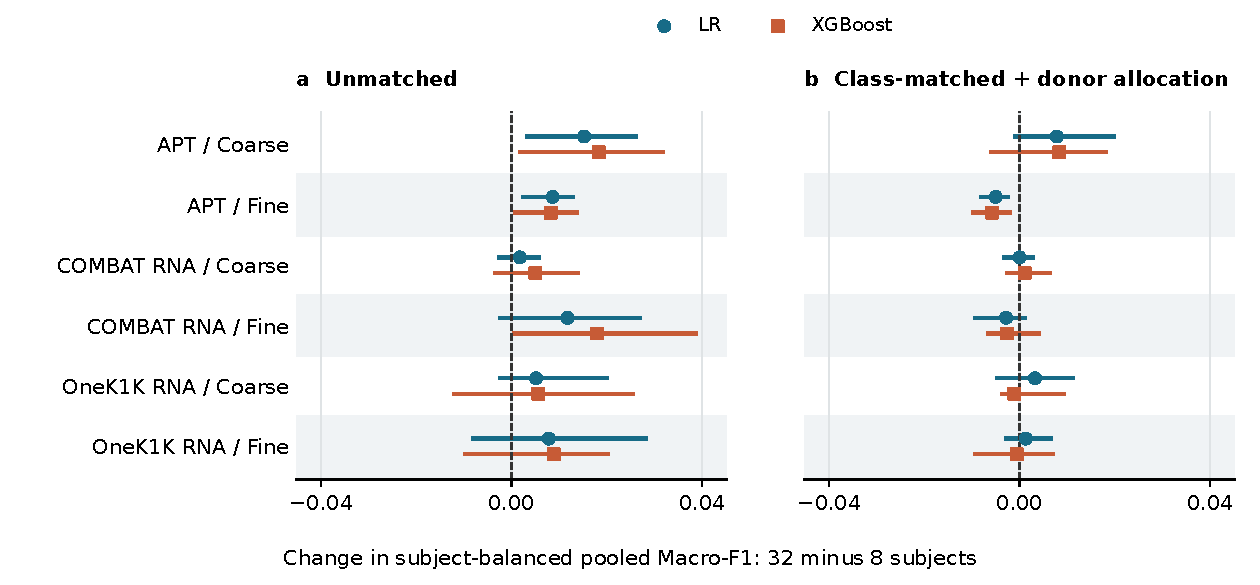
\includegraphics[width=\columnwidth]{figures/scaling_protocol_contrast.pdf}
\caption{The apparent breadth advantage changes under the matched protocol.
Both panels show the change in subject-balanced pooled OOF macro-F1 from 8 to
32 training subjects at $T=6{,}400$, on identical axes. The right panel fixes
class support and exact quotas and additionally uses within-class donor round
robin; this is not a label-only intervention. Points are seed means; bars in
both panels are empirical 2.5th--97.5th seed percentiles, not confidence
intervals of the mean. Unmatched runs and matched LR use 20 seeds; matched
XGBoost uses 10. APT and COMBAT fine point estimates change sign for both models.
Cross-panel changes are descriptive, not paired attenuation tests. The matched
joint stability intervals, which additionally resample held-out subjects, all span zero
(Figure~\ref{fig:class_matched_joint}).}
\label{fig:class_matched_scaling}
\end{figure}

The matched policy yields a different pattern
(Figure~\ref{fig:class_matched_scaling}). At $T=6{,}400$, LR/XGBoost effects
are $+0.0078/+0.0083$ for APT coarse but $-0.0050/-0.0058$ for APT fine.
COMBAT effects are approximately zero for coarse and $-0.0028/-0.0027$ for
fine. OneK1K effects are small and change sign across models. All 12 joint
stability intervals include zero. The APT and COMBAT fine point-estimate
reversals are therefore not specific to a linear classifier, but their signs
are not stable across joint resampling. This is a
joint sampling-protocol contrast: the implementation fixes observed labels,
class counts, and proportions and also uses within-class donor round robin.
The attenuation cannot therefore be assigned solely to label distribution.
An independently controlled synthetic check separates quota matching from donor
allocation (Section~\ref{sec:appendix:sequential_simulation}). The completed
real-cohort separation in Section~\ref{sec:sequential_completed} retains
positive fine effects under exact quotas alone, demonstrating the importance
of distinguishing quota matching from donor allocation. A complementary known-null
validation yields mean effects $+0.0202$, $+0.0119$, and $+0.0004$ for unmatched,
support-matched, and exact-quota sampling against an exactly zero overlap-quota
target. Independent Monte Carlo references under donor shifts remain positive
and are not mechanically removed by matching
(Section~\ref{sec:appendix:known_target}). This checks recovery of a specified
allocation target, not interval coverage or a universal causal effect of subject breadth.

Beyond the common 32-subject grid, class-matched LR
frontiers through 64 COMBAT and 128 OneK1K training donors yield adjacent
mean effects between $-0.00065$ and $+0.00123$, with every joint stability interval
spanning zero. These ranges do not test mean equivalence or a plateau. A post-hoc
$\pm0.01$ sensitivity band contains 11 of 12 adjacent frontier stability intervals,
but only 4 of 12 main $T=6{,}400$ intervals and none of the four APT intervals
(Section~\ref{sec:appendix:equivalence}). These are pointwise interval-containment
diagnostics, not equivalence tests or an optimal-allocation result. Complete unmatched
grids, class-support audits, matched doublings, extended frontiers, and
uncertainty decompositions appear in
Section~\ref{sec:appendix:fair_scaling}--
\ref{sec:appendix:extended_subject_frontier}.


\subsection{Fair Fixed-Total and Matched-Scale Analysis}
\label{sec:appendix:fair_scaling}

The supporting scaling design uses $P\in\{8,16,32\}$ and
$C\in\{100,200,400,800,1600\}$, with 20 nested subset seeds for every outer
fold. Because every retained patient has at least 1{,}929 cells, all finite caps
are feasible without replacement. Disease-stratified patient orderings are
nested across $P$, uniform cell permutations are nested across $C$, no subtype
label enters sampling, and preprocessing is refit on each sampled training set.
The fixed-total diagonals satisfy $PC\in\{3200,6400,12800\}$ exactly.

\input{tables/fixed_total_scaling}

\begin{figure}[H]
\centering
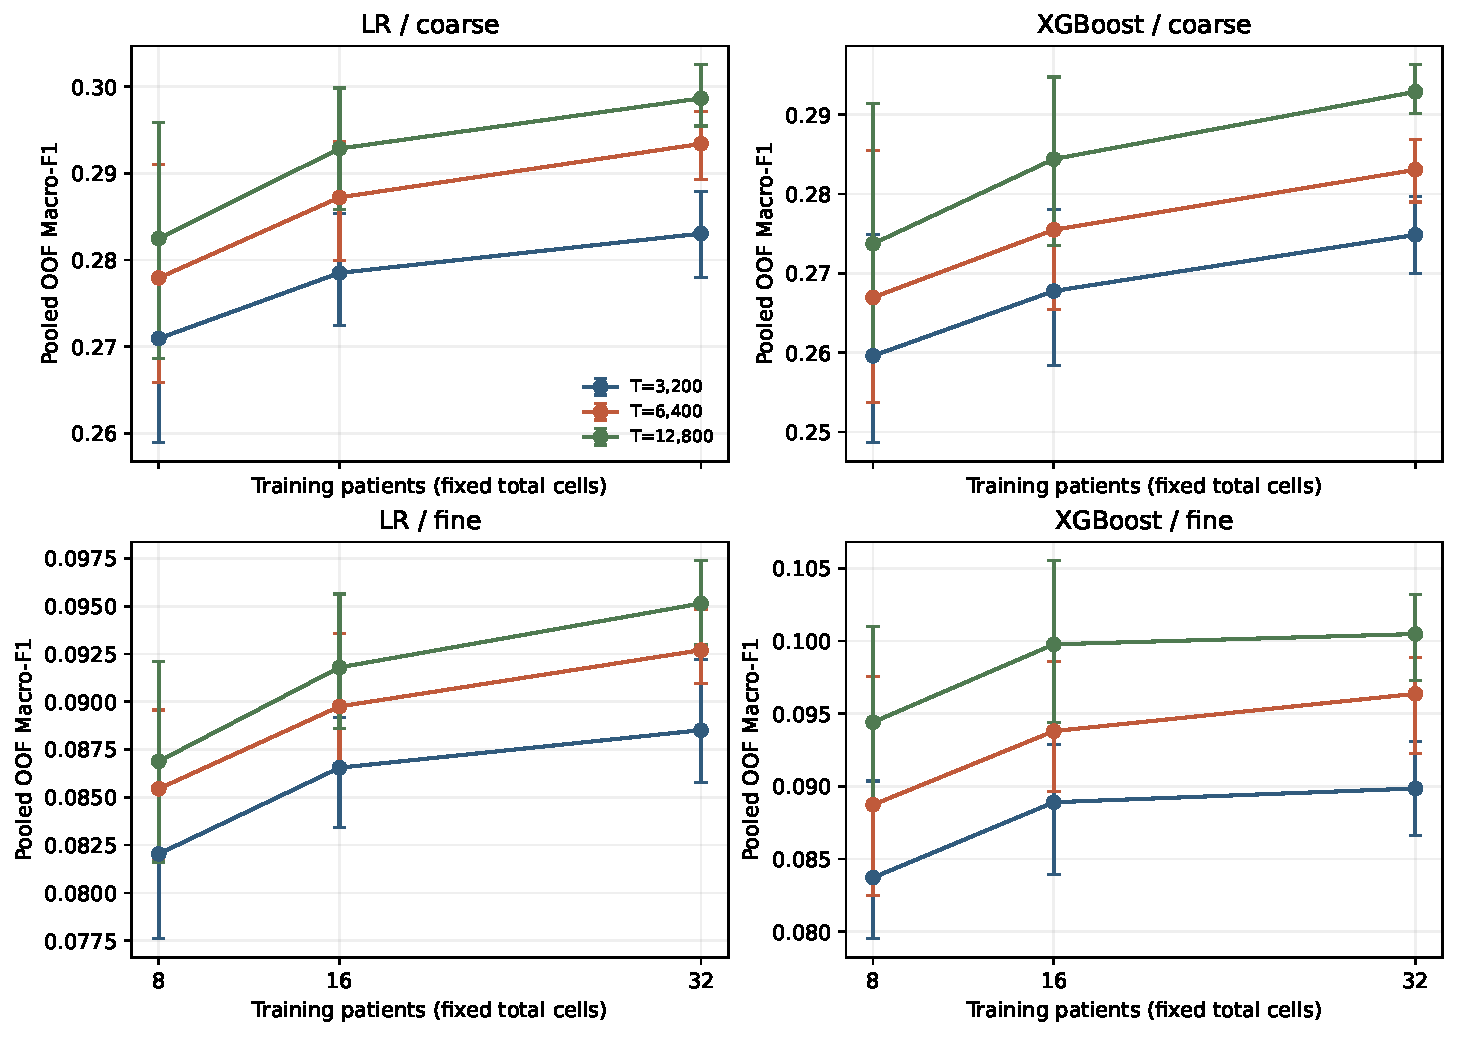
\includegraphics[width=0.92\textwidth]{figures/fixed_total_scaling.pdf}
\caption{APT-only fixed-total response curves underlying the unmatched
cross-cohort diagnostic in Table~\ref{tab:cross_cohort_scaling}. Points are pooled OOF
macro-F1 means over 20 matched subset seeds; bars are empirical 95\% seed
intervals. Patient-balanced and patient-bootstrap results are provided in the
machine-readable artifacts.}
\label{fig:apt_fixed_total_scaling}
\end{figure}

Table~\ref{tab:fixed_total_scaling} reports variability across subset seeds.
Separately, paired patient-clustered bootstraps over the same 40 pooled OOF
patients compare $P=8$ with $P=32$ after averaging seed-level sufficient
statistics. All 12 intervals exclude zero; their lower endpoints range from
0.0002 to 0.0084 and upper endpoints from 0.0090 to 0.0314. These intervals
quantify uncertainty over patients, whereas the empirical seed intervals
quantify sensitivity to which development patients and cells are sampled.

Matched doubling effects average patient versus cell gains of
0.011/0.005 (LR coarse), 0.007/0.003 (LR fine), 0.016/0.008 (XGBoost coarse),
and 0.009/0.006 (XGBoost fine). In the descriptive fold-fixed-effect response
surface, the corresponding per-doubling $\beta_P/\beta_C$ coefficients are
0.017/0.008, 0.008/0.004, 0.016/0.007, and 0.009/0.006. Complete pairwise
effects, patient intervals, seed intervals, and response-surface uncertainty
are stored in the machine-readable scaling artifacts. The coefficients are
associations over this grid, not causal or universal scaling laws.

\subsection{External COMBAT and OneK1K Scaling Replications}
\label{sec:appendix:combat_scaling}

We downloaded the author-released COMBAT CITE-seq object
\citep{combat2022blood} (836{,}148 cells and 124 donor identifiers; SHA-256
\texttt{f628a15f25b9ca2f7cdefeab271fd9d007c8d5e47eb80c4b807d5f65e86ff53d}).
We removed cells without a resolved major or fine immune annotation and cells
flagged as GEX-region doublets. Ten donors were frozen as a calibration-only
set and excluded from every model fit and test fold. Among the remaining
donors, requiring at least 1{,}600 eligible cells leaves 105 donors and
700{,}706 cells. We construct five disjoint folds of 21 test donors, stratified
by the released sample-source field, and freeze these folds across all models,
budgets, seeds, and modalities.

The RNA replication uses 293 protein-coding genes with highest variance on the
10 calibration donors after excluding mitochondrial and ribosomal genes. This
matches the APT input dimension without selecting features on any evaluation
donor. The ADT sensitivity uses all 192 released antibody features. Both inputs
use the released five-class major annotation and 39-class fine annotation.
They share the exact $P$, $C$, and fixed-total grids, 20 nested source-stratified
donor/cell seeds, training-only standardization, LR configuration, and paired
donor-bootstrap procedure used in APT-Bench. The RNA analysis additionally
uses the frozen 400-tree XGBoost baseline. Every fit is evaluated on all cells
of the 21 untouched test donors; the ADT analysis is an LR-only modality
sensitivity rather than an additional model-comparison family. Dataset hashes,
folds, features, sampling manifests, and per-donor sufficient statistics are
included in the release artifacts.

OneK1K provides a second independent scRNA-seq replication in a much larger
healthy PBMC cohort \citep{yazar2022onek1k}. We use the current author-deposited
CELLxGENE object (1{,}248{,}980 cells and 981 donor identifiers; SHA-256
\texttt{14c5e9e70007a5e7dc047f7b29405773305e1a7b9791d0789af70649cf6f46ec}),
remove released doublet calls, and reserve one complete multiplexing pool for
calibration. Requiring at least 800 eligible cells leaves 925 evaluation donors
and 1{,}199{,}468 cells. Five folds are disjoint in both donor and multiplexing
pool. We select 293 protein-coding, non-mitochondrial, non-ribosomal genes by
variance on ten calibration-pool donors only, and use the released 30-class
Azimuth-derived fine labels with a deterministic five-lineage mapping.

OneK1K uses the same models, 20 nested subset seeds, training-only
standardization, untouched-test-donor evaluation, subject-balanced pooled metric, and
2{,}000 paired donor bootstraps. Its grid is
$P\in\{8,16,32\}$ and $C\in\{100,200,400,800\}$, yielding the two common exact
budgets $T\in\{3200,6400\}$. We prespecified the lower depth ceiling because
only 116 of the 981 raw donors have at least 1{,}600 eligible cells; enforcing
the full APT grid would discard most donors and condition the replication on
high cell recovery. OneK1K tests scaling portability in a healthy cohort, not
disease generalization or absolute accuracy across different feature spaces
and label-generation procedures.

\begin{table}[H]
\centering
\small
\setlength{\tabcolsep}{3.5pt}
\resizebox{\textwidth}{!}{%
\begin{tabular}{lllrrr}
\toprule
Dataset & Modality & Model/task & $T=3{,}200$ & $T=6{,}400$ & $T=12{,}800$ \\
\midrule
APT & Aptamer & LR/Coarse & +0.012 [+0.005, +0.021] & +0.015 [+0.007, +0.024] & +0.017 [+0.009, +0.026] \\
APT & Aptamer & LR/Fine & +0.008 [+0.004, +0.011] & +0.009 [+0.005, +0.012] & +0.010 [+0.005, +0.013] \\
APT & Aptamer & XGBoost/Coarse & +0.017 [+0.008, +0.027] & +0.018 [+0.007, +0.030] & +0.022 [+0.009, +0.035] \\
APT & Aptamer & XGBoost/Fine & +0.007 [+0.002, +0.011] & +0.008 [+0.002, +0.013] & +0.006 [+0.000, +0.011] \\
COMBAT & RNA & LR/Coarse & +0.003 [+0.002, +0.004] & +0.002 [+0.001, +0.003] & +0.001 [+0.001, +0.002] \\
COMBAT & RNA & LR/Fine & +0.012 [+0.009, +0.013] & +0.012 [+0.010, +0.012] & +0.007 [+0.005, +0.009] \\
COMBAT & RNA & XGBoost/Coarse & +0.006 [+0.005, +0.007] & +0.005 [+0.004, +0.006] & +0.004 [+0.003, +0.005] \\
COMBAT & RNA & XGBoost/Fine & +0.016 [+0.013, +0.017] & +0.018 [+0.016, +0.019] & +0.017 [+0.014, +0.018] \\
COMBAT & ADT & LR/Coarse & +0.006 [+0.004, +0.008] & +0.009 [+0.006, +0.012] & +0.012 [+0.010, +0.016] \\
COMBAT & ADT & LR/Fine & +0.013 [+0.010, +0.014] & +0.011 [+0.010, +0.013] & +0.011 [+0.009, +0.013] \\
OneK1K & RNA & LR/Coarse & +0.004 [+0.004, +0.005] & +0.005 [+0.005, +0.006] & -- \\
OneK1K & RNA & LR/Fine & +0.007 [+0.007, +0.009] & +0.008 [+0.007, +0.009] & -- \\
OneK1K & RNA & XGBoost/Coarse & -0.003 [-0.004, -0.002] & +0.006 [+0.005, +0.006] & -- \\
OneK1K & RNA & XGBoost/Fine & +0.006 [+0.005, +0.007] & +0.009 [+0.007, +0.009] & -- \\
\bottomrule
\end{tabular}
}
\caption{Unmatched diagnostic: change in subject-balanced, subject-disjoint OOF Macro-F1 when the same total training-cell budget is reallocated from 8 to 32 independent subjects without freezing the marginal training label distribution. Brackets are 95\% paired subject-bootstrap intervals over the fixed outer-test subjects. Positive values favor broader subject coverage but can also reflect changes in observed classes, per-class counts, and class proportions. COMBAT ADT is a prespecified modality sensitivity using LR only. OneK1K uses the two common exact budgets supported by at least 800 cells from nearly all donors.}
\label{tab:cross_cohort_scaling}
\end{table}


\subsection{Label-Distribution Audit and Matched Control}
\label{sec:appendix:class_matched_scaling}

The label-agnostic grid samples cells uniformly within subjects and therefore
allows the full marginal label distribution to vary. Machine-readable audit tables report the
observed class count, unseen-at-training class count, cell count, and donor
count for every class at every fold, seed, and scaling point. The main text
reports the common fixed-total diagonals, where fine-class coverage increases
slightly with $P$ despite fixed $T$; this coverage statistic is only one
observable component of the broader label-distribution effect.

The class-matched control fixes the marginal label distribution. The $P=8$ subset defines the
observed labels and a proportional integer quota $T_k$ with a one-cell floor;
capacity violations are deterministically redistributed. The same quota vector
is then used at $P=8,16,32$. Within each class, a capacity-constrained
round-robin sampler distributes cells across selected subjects before assigning
a second cell from the same subject, so increasing $P$ changes realized donor
coverage rather than class counts. Sampling is without replacement,
standardization is refit on each training subset, and all immutable outer-test
cells are retained. All three runs complete 1{,}200/1{,}200 jobs and pass checks
for exact total cells, identical paired class counts, non-overlapping test
subjects, and contribution by every nominal training subject.
These primary Logistic Regression runs use 20 matched subset seeds at both
$T=3{,}200$ and $T=6{,}400$. To test whether the matched-policy direction is specific
to a linear classifier, we repeat the identical control with the frozen XGBoost
configuration at $T=6{,}400$ using 10 matched seeds. Each dataset completes
300/300 additional jobs and passes the same checks; final production fits use
the CPU histogram backend throughout to avoid mixing computational backends.
It does not separately identify changes in disease--subtype composition,
within-class allocation across subjects, or within-class subject heterogeneity;
these remain bundled with the subject-breadth intervention.

\begin{table}[H]
\centering
\small
\setlength{\tabcolsep}{4pt}
\resizebox{\textwidth}{!}{%
\begin{tabular}{llrrcc}
\toprule
Dataset & Task & $T$ & Classes (mean/total) & Donors/class ($P$: 8$\rightarrow$32) & $\Delta$ subject-balanced M-F1 \\
\midrule
APT & Coarse & 3,200 & 5.0/5 & 7.9$\rightarrow$28.5 & +0.0062 [+0.0008, +0.0129] \\
APT & Coarse & 6,400 & 5.0/5 & 7.9$\rightarrow$30.5 & +0.0078 [+0.0022, +0.0160] \\
APT & Fine & 3,200 & 26.8/27 & 7.1$\rightarrow$25.0 & -0.0024 [-0.0042, -0.0004] \\
APT & Fine & 6,400 & 26.8/27 & 7.2$\rightarrow$27.4 & -0.0050 [-0.0068, -0.0026] \\
COMBAT RNA & Coarse & 3,200 & 5.0/5 & 8.0$\rightarrow$29.0 & +0.0011 [+0.0005, +0.0017] \\
COMBAT RNA & Coarse & 6,400 & 5.0/5 & 8.0$\rightarrow$31.3 & +0.0000 [-0.0004, +0.0004] \\
COMBAT RNA & Fine & 3,200 & 39.0/39 & 7.2$\rightarrow$22.5 & -0.0007 [-0.0014, +0.0006] \\
COMBAT RNA & Fine & 6,400 & 39.0/39 & 7.3$\rightarrow$26.6 & -0.0028 [-0.0037, -0.0018] \\
OneK1K RNA & Coarse & 3,200 & 5.0/5 & 7.8$\rightarrow$27.7 & +0.0025 [+0.0020, +0.0031] \\
OneK1K RNA & Coarse & 6,400 & 5.0/5 & 7.8$\rightarrow$29.6 & +0.0033 [+0.0026, +0.0039] \\
OneK1K RNA & Fine & 3,200 & 29.0/30 & 6.2$\rightarrow$19.8 & +0.0019 [+0.0010, +0.0030] \\
OneK1K RNA & Fine & 6,400 & 29.0/30 & 6.4$\rightarrow$22.1 & +0.0013 [+0.0002, +0.0023] \\
\bottomrule
\end{tabular}
}
\caption{Class-matched fixed-total control using class-weighted multinomial Logistic Regression. Within each outer-fold/seed/task pair, the $P=8$ subset freezes the observed classes and exact per-class cell quotas; the same quotas are used at $P=16$ and $P=32$. Brackets are 95\% paired subject-bootstrap intervals after averaging the 20 seed-level sufficient statistics; empirical seed intervals are released separately. Donors/class reports the mean number of subjects contributing cells to an observed class.}
\label{tab:class_matched_scaling}
\end{table}


\begin{figure}[tbp]
\centering
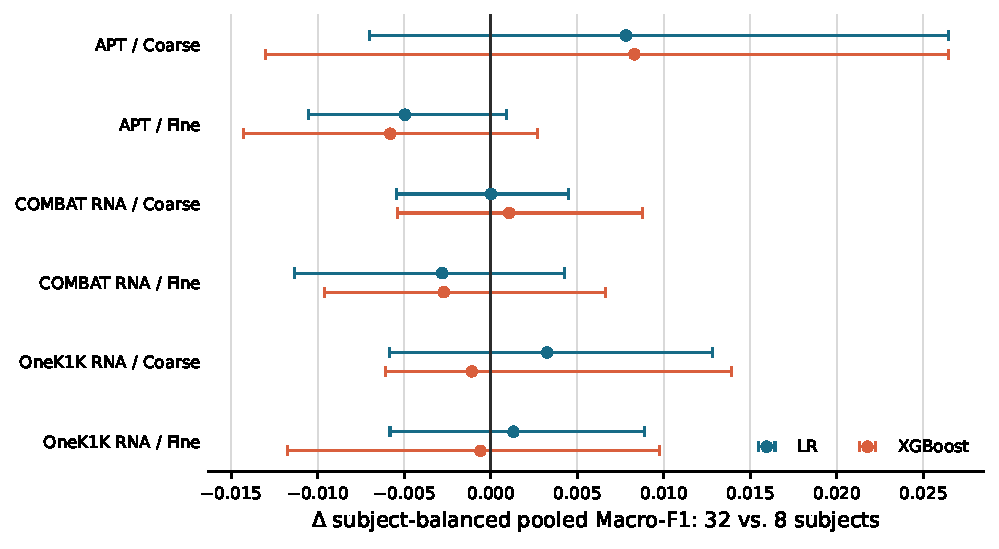
\includegraphics[width=0.80\columnwidth]{figures/class_matched_scaling.pdf}
\caption{Joint stability for the completed class-matched protocol at
$T=6{,}400$. Points are mean changes in subject-balanced pooled OOF macro-F1
from 8 to 32 subjects. The 95\% joint stability intervals select one training-subset seed
and bootstrap paired held-out subjects; all 12 span zero. Unlike the seed-only
bars in Figure~\ref{fig:class_matched_scaling}, these intervals include test-subject
variability. They are not confidence intervals for the seed-averaged effect;
zero inclusion does not test a zero mean or establish equivalence.}
\label{fig:class_matched_joint}
\end{figure}

The primary stability diagnostic combines both variation sources. In each of 2{,}000
replicates, we sample one completed training-subset seed uniformly, resample
outer-test subjects with replacement, use the same subject draw for $P=8$ and
$P=32$, and recompute the paired difference. All 18 joint 95\% stability intervals
include zero, and the table reports the empirical positive-replicate fraction. For
decomposition, empirical seed-only intervals include zero in 16 of 18 rows;
the exceptions are the two negative APT fine results at $T=6{,}400$.
Subject-only intervals condition on the seed-averaged prediction matrix and can
exclude zero even when the joint stability interval does not. The constructions
answer different questions: the joint range retains variation between fitted
training subsets rather than estimating uncertainty of their average. Neither
zero inclusion nor the positive-replicate fraction is a test of the mean effect.
These ranges also lack a demonstrated coverage guarantee for a future training
cohort; they are conditional resampling diagnostics.

\subsection{Extended External Subject Frontier}
\label{sec:appendix:extended_subject_frontier}

The common $P\leq32$ grid is imposed by the 40-patient APT cohort, not by the
capacity of the external datasets. We therefore extend the class-matched LR
control to $P=64$ for COMBAT and to $P\in\{64,128\}$ for OneK1K at
$T\in\{3{,}200,6{,}400\}$. The original $P=8$ subset freezes the class set and
integer per-class quotas for every fold, seed, task, and total; only the number
of selected subjects allowed to contribute those cells changes. Each new point
uses 10 nested subset seeds, all immutable outer-test subjects, and the same
joint resampling of training-subset seed and held-out subjects used in the
primary matched control. This extension is an external-cohort allocation
sensitivity rather than a claim that its largest tested $P$ is globally
optimal.

\begin{figure}[H]
\centering
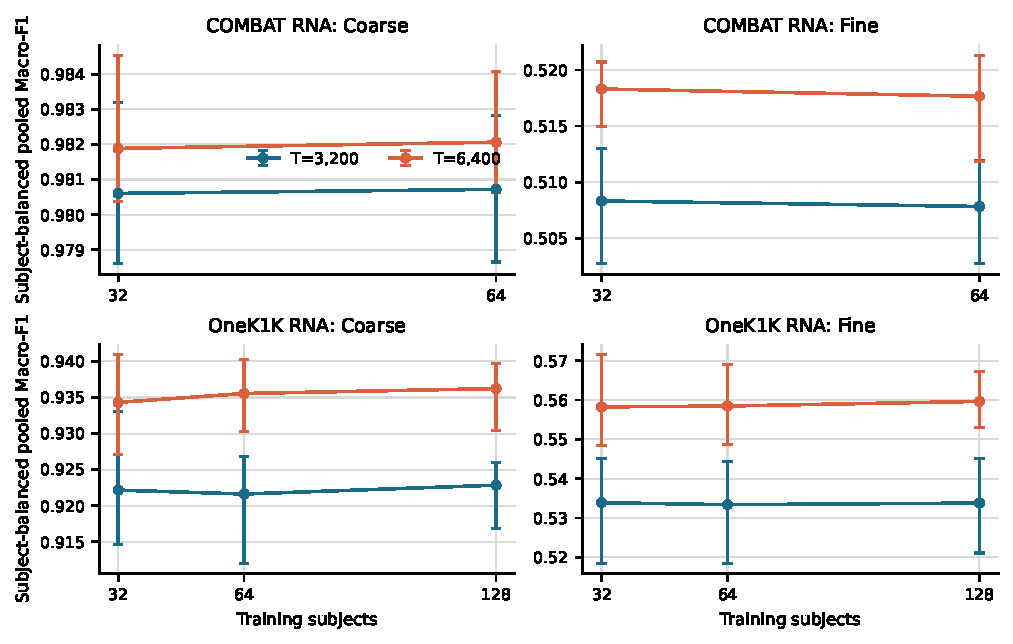
\includegraphics[width=0.86\textwidth]{figures/extended_subject_frontier.pdf}
\caption{Class-matched LR frontier beyond 32 training subjects. Points are
mean subject-balanced pooled OOF macro-F1 over 10 matched training-subset seeds; bars
are empirical 95\% seed intervals and therefore visualize subset sensitivity,
not uncertainty of the mean. The paired joint stability intervals are
reported in Table~\ref{tab:extended_subject_frontier}.}
\label{fig:extended_subject_frontier}
\end{figure}

\begin{table}[H]
\centering
\small
\setlength{\tabcolsep}{5pt}
\begin{tabular}{llrrcc}
\toprule
Dataset & Task & $T$ & Subjects & $\Delta$ SB-pooled M-F1 & $\Pr(\Delta>0)$ \\
\midrule
COMBAT RNA & Coarse & 3,200 & 32$\rightarrow$64 & +0.0001 [-0.0020, +0.0025] & 0.535 \\
COMBAT RNA & Coarse & 6,400 & 32$\rightarrow$64 & +0.0002 [-0.0014, +0.0016] & 0.618 \\
COMBAT RNA & Fine & 3,200 & 32$\rightarrow$64 & -0.0005 [-0.0060, +0.0026] & 0.498 \\
COMBAT RNA & Fine & 6,400 & 32$\rightarrow$64 & -0.0006 [-0.0060, +0.0040] & 0.450 \\
\midrule
OneK1K RNA & Coarse & 3,200 & 32$\rightarrow$64 & -0.0005 [-0.0111, +0.0052] & 0.553 \\
OneK1K RNA & Coarse & 6,400 & 32$\rightarrow$64 & +0.0012 [-0.0046, +0.0046] & 0.766 \\
OneK1K RNA & Fine & 3,200 & 32$\rightarrow$64 & -0.0005 [-0.0060, +0.0053] & 0.418 \\
OneK1K RNA & Fine & 6,400 & 32$\rightarrow$64 & +0.0002 [-0.0096, +0.0063] & 0.595 \\
OneK1K RNA & Coarse & 3,200 & 64$\rightarrow$128 & +0.0012 [-0.0023, +0.0068] & 0.642 \\
OneK1K RNA & Coarse & 6,400 & 64$\rightarrow$128 & +0.0007 [-0.0042, +0.0043] & 0.657 \\
OneK1K RNA & Fine & 3,200 & 64$\rightarrow$128 & +0.0004 [-0.0039, +0.0050] & 0.542 \\
OneK1K RNA & Fine & 6,400 & 64$\rightarrow$128 & +0.0012 [-0.0066, +0.0068] & 0.617 \\
\bottomrule
\end{tabular}
\caption{Extended class-matched subject frontier for Logistic Regression. Each comparison holds the total training-cell budget, observed class set, and exact per-class cell quotas fixed while increasing the number of contributing training subjects. Values are paired mean changes; brackets are joint 95\% stability intervals from 2{,}000 replicates that sample a matched training-subset seed and then bootstrap held-out subjects. The final column is the empirical fraction of positive replicates, not a posterior probability. These ranges are not confidence intervals for seed-averaged effects.}
\label{tab:extended_subject_frontier}
\end{table}


All 12 adjacent frontier effects are small: their means range from $-0.00065$
to $+0.00123$, and every joint stability interval includes zero. The four direct OneK1K
$32\rightarrow128$ contrasts likewise span zero under joint resampling. This does not
establish a plateau or exclude practically meaningful changes. The explicit
margin sensitivity below assesses interval width separately from zero inclusion.
Because the intervention remains tied to these tasks, budgets, features, and LR
configuration, it does not locate a universal saturation point or optimal allocation.

\subsection{Post-Hoc Stability-Band Sensitivity}
\label{sec:appendix:equivalence}

Failure to detect a difference is not evidence of equivalence
\citep{lakens2017equivalence}. After inspecting the existing results, we add an
\emph{exploratory} smallest-effect sensitivity bound $\epsilon=0.01$ absolute
subject-balanced pooled Macro-F1 (one percentage point), with $0.005$ and $0.02$
as sensitivity values. This is a reporting tolerance, not a validated clinical
threshold, and was not prespecified for the completed experiments. It must not
be conflated with the separate compact-panel tolerance $\delta=0.02$.

For each released joint 95\% stability interval $[L,U]$, we report zero inclusion
($L\leq0\leq U$) and strict containment ($-\epsilon<L$ and $U<\epsilon$)
separately. Containment describes concentration of this conditional resampling
distribution inside the chosen band, not equivalence of the mean allocation
effects. Intervals with $L\leq-\epsilon$ and $U\geq\epsilon$ span changes of
the stated magnitude in both directions. These diagnostics neither quantify
statistical power nor provide a calibrated future-cohort guarantee.

\begin{table}[htbp]
\centering\small
\begin{tabular}{lllrrrrr}
\toprule
Comparison & Dataset & Task & $n$ & $\pm .005$ & $\pm .010$ & $\pm .020$ & Both signs$^*$ \\
\midrule
8--32 & APT & coarse & 2 & 0 & 0 & 0 & 1 \\
8--32 & APT & fine & 2 & 0 & 0 & 2 & 0 \\
8--32 & COMBAT & coarse & 2 & 0 & 2 & 2 & 0 \\
8--32 & COMBAT & fine & 2 & 0 & 1 & 2 & 0 \\
8--32 & OneK1K & coarse & 2 & 0 & 0 & 2 & 0 \\
8--32 & OneK1K & fine & 2 & 0 & 1 & 2 & 0 \\
Extended LR & COMBAT & coarse & 2 & 2 & 2 & 2 & 0 \\
Extended LR & COMBAT & fine & 2 & 0 & 2 & 2 & 0 \\
Extended LR & OneK1K & coarse & 4 & 2 & 3 & 4 & 0 \\
Extended LR & OneK1K & fine & 4 & 0 & 4 & 4 & 0 \\
\bottomrule
\end{tabular}
\caption{Post-hoc practical-equivalence sensitivity: number of released joint 95\% intervals strictly inside each stated margin. The 8--32 rows use $T=6{,}400$ and both LR and XGBoost; extended rows use LR at both totals for adjacent subject-budget comparisons. $^*$Intervals reaching both $-0.01$ and $+0.01$, indicating insufficient precision to exclude meaningful effects in either direction. Counts are pointwise diagnostics, not formal TOST decisions or evidence that an entire scaling frontier is equivalent.}
\label{tab:equivalence_sensitivity}
\end{table}


At $T=6{,}400$, only 4 of 12 main comparison intervals meet the $\pm0.01$
containment criterion; none of the four APT intervals does. The APT coarse
XGBoost interval spans both meaningful directions. Among adjacent external LR
frontier comparisons, 11 of 12 intervals meet this criterion; the exception is
OneK1K coarse $32\rightarrow64$ at $T=3{,}200$. With the tighter $\pm0.005$
margin, no main interval and only 4 of 12 adjacent frontier intervals are
contained. Descriptive stability is therefore margin-dependent; these counts
do not establish that the sampling policies are equivalent or subjects have no value.

We do not report formal TOST $p$-values. Conventional level-0.05 TOST is linked
to a corresponding 90\% confidence interval, whereas this analysis retains the
released joint 95\% stability intervals. More fundamentally, those intervals sample one completed
training-subset seed and then test subjects, combining between-fit variability
with test uncertainty rather than estimating only a seed-averaged mean effect.
Containment is therefore an exploratory joint-interval screen, not a calibrated
confirmatory equivalence test. Results are pointwise, without a simultaneous
equivalence guarantee across rows, and do not establish a continuous plateau
between or beyond the tested budgets. This audit concerns the completed legacy
controls, not the ongoing A--D GPU rerun.

\subsection{Secondary Descriptive Patient--Cell Scaling Surface}
\label{sec:appendix:patient_cell_scaling}

This historical $4\times4$ surface fixes eight outer-test patients and varies only the training
set. For each outer fold and each of 20 seeds, we generate one approximately
proportional disease-stratified ordering of the 32 development patients, giving
nested sets $S_8\subset S_{16}\subset S_{24}\subset S_{32}$. Each selected
patient receives one uniform random cell ordering, giving nested prefixes of
100, 500, and 2{,}000 cells and the complete available set. Patients with fewer
than a requested cap contribute all available cells. No cell is selected using
its subtype, and every model is evaluated on all cells from the untouched test
patients. The full-data endpoint is fitted once per fold rather than duplicated
across seeds. All 6{,}020 model--task jobs completed, and the deterministic
endpoint exactly reproduces the frozen pooled OOF baselines within absolute
tolerance $5\times10^{-4}$. Because $P{=}8\rightarrow32$ is a fourfold change
whereas $C{=}100\rightarrow\mathrm{all}$ is a larger and patient-dependent
change, this surface is descriptive only. All direct comparisons between the
two axes use the fixed-total and matched-doubling analysis in the main paper.

\begin{table*}[t]
\centering
\scriptsize
\resizebox{\textwidth}{!}{%
\begin{tabular}{llrrrr}
\toprule
Model & Task & $C=100$ & $C=500$ & $C=2000$ & $C=\mathrm{all}$ \\
\midrule
Logistic Regression, $P=8$ & Coarse & 0.255 [0.247, 0.265] & 0.274 [0.263, 0.284] & 0.283 [0.269, 0.297] & 0.282 [0.269, 0.293] \\
Logistic Regression, $P=16$ & Coarse & 0.266 [0.261, 0.270] & 0.290 [0.284, 0.297] & 0.288 [0.282, 0.295] & 0.290 [0.280, 0.300] \\
Logistic Regression, $P=24$ & Coarse & 0.276 [0.269, 0.280] & 0.296 [0.288, 0.304] & 0.288 [0.282, 0.295] & 0.296 [0.289, 0.302] \\
Logistic Regression, $P=32$ & Coarse & 0.283 [0.278, 0.288] & 0.299 [0.296, 0.302] & 0.287 [0.284, 0.288] & 0.299 [0.284, 0.315] \\
Logistic Regression, $P=8$ & Fine & 0.074 [0.068, 0.081] & 0.084 [0.079, 0.088] & 0.087 [0.082, 0.092] & 0.101 [0.091, 0.109] \\
Logistic Regression, $P=16$ & Fine & 0.081 [0.078, 0.085] & 0.090 [0.088, 0.094] & 0.095 [0.090, 0.099] & 0.116 [0.110, 0.125] \\
Logistic Regression, $P=24$ & Fine & 0.086 [0.083, 0.089] & 0.093 [0.089, 0.097] & 0.100 [0.095, 0.105] & 0.125 [0.118, 0.131] \\
Logistic Regression, $P=32$ & Fine & 0.089 [0.086, 0.092] & 0.095 [0.093, 0.097] & 0.105 [0.102, 0.108] & 0.132 [0.112, 0.146] \\
\midrule
XGBoost, $P=8$ & Coarse & 0.246 [0.234, 0.263] & 0.262 [0.250, 0.278] & 0.277 [0.262, 0.293] & 0.300 [0.283, 0.321] \\
XGBoost, $P=16$ & Coarse & 0.260 [0.252, 0.272] & 0.278 [0.268, 0.288] & 0.295 [0.283, 0.306] & 0.313 [0.298, 0.330] \\
XGBoost, $P=24$ & Coarse & 0.270 [0.264, 0.276] & 0.289 [0.284, 0.295] & 0.305 [0.297, 0.312] & 0.319 [0.311, 0.328] \\
XGBoost, $P=32$ & Coarse & 0.275 [0.270, 0.280] & 0.296 [0.293, 0.298] & 0.310 [0.308, 0.312] & 0.322 [0.300, 0.345] \\
XGBoost, $P=8$ & Fine & 0.073 [0.068, 0.079] & 0.085 [0.080, 0.091] & 0.096 [0.090, 0.103] & 0.118 [0.110, 0.126] \\
XGBoost, $P=16$ & Fine & 0.082 [0.077, 0.085] & 0.096 [0.092, 0.101] & 0.110 [0.103, 0.120] & 0.132 [0.125, 0.140] \\
XGBoost, $P=24$ & Fine & 0.087 [0.081, 0.092] & 0.100 [0.095, 0.104] & 0.115 [0.110, 0.121] & 0.138 [0.132, 0.144] \\
XGBoost, $P=32$ & Fine & 0.090 [0.087, 0.093] & 0.102 [0.100, 0.105] & 0.118 [0.117, 0.121] & 0.143 [0.127, 0.159] \\
\midrule
\bottomrule
\end{tabular}
}
\caption{Patient--cell training scaling. Entries are pooled OOF Macro-F1 means with empirical 2.5th--97.5th seed intervals; the deterministic $P=32,C=\mathrm{all}$ endpoint instead uses a patient-clustered bootstrap interval. Seed intervals are not patient confidence intervals.}
\label{tab:patient_cell_scaling}
\end{table*}


\begin{figure}[H]
\centering
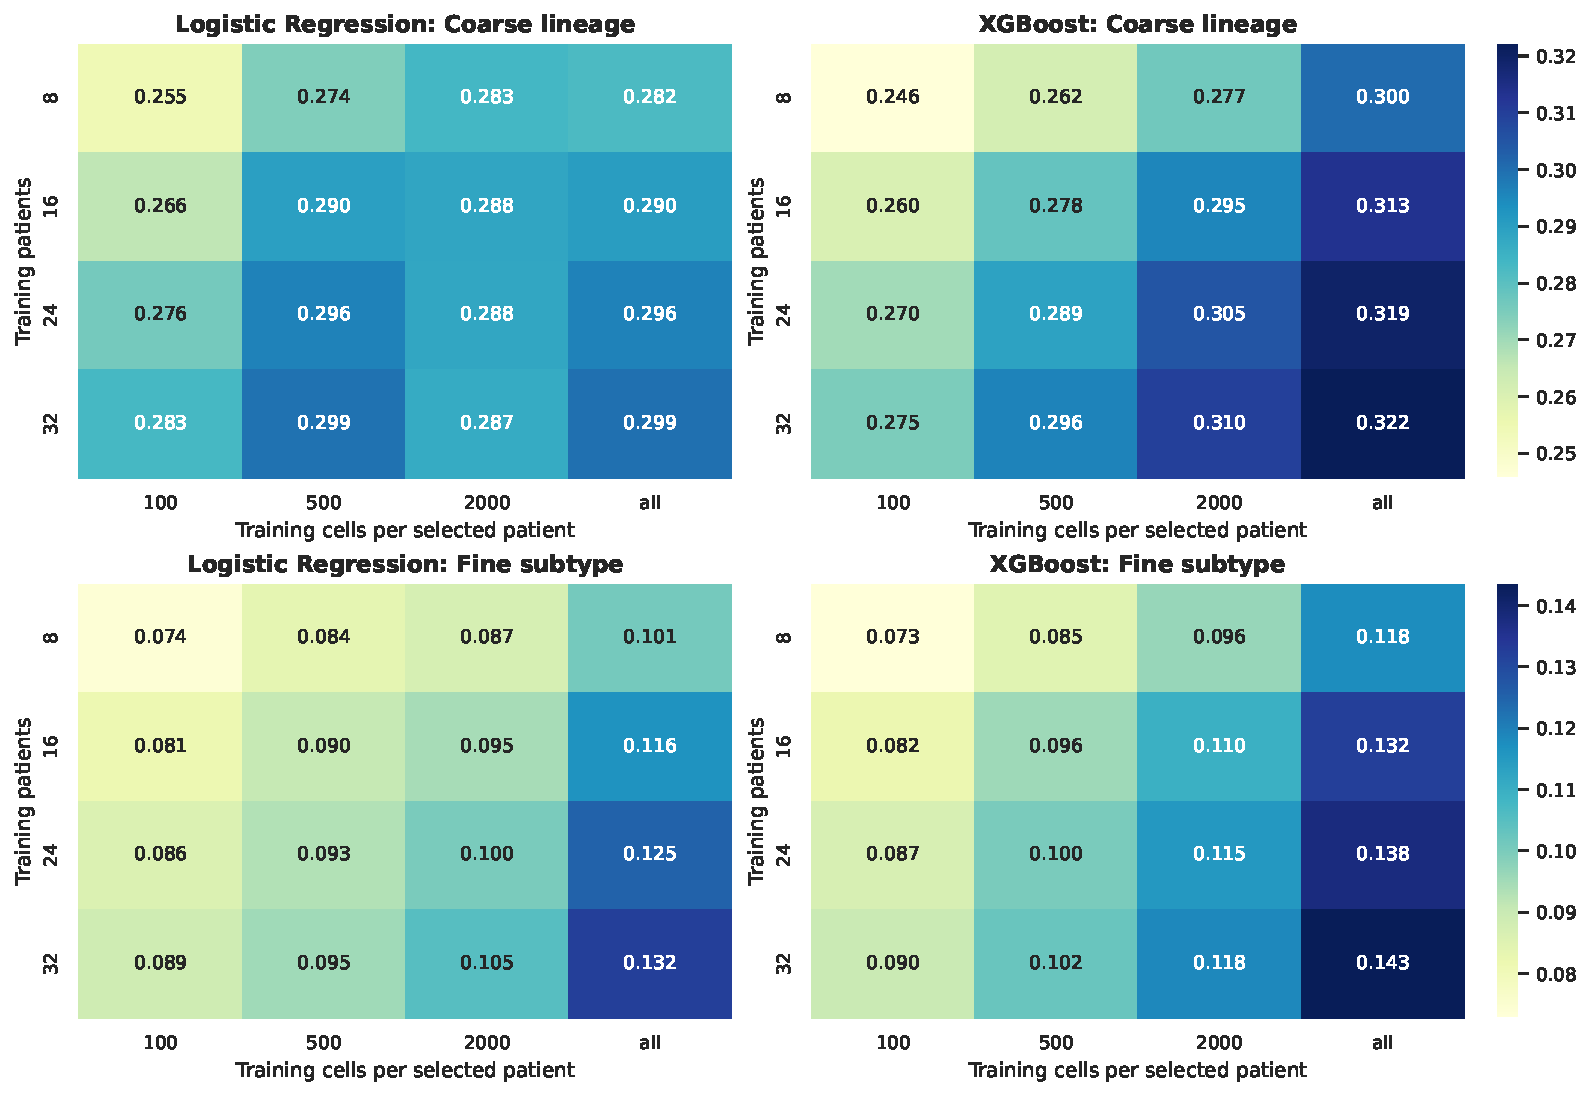
\includegraphics[width=\textwidth]{figures/patient_cell_scaling_heatmaps.pdf}
\caption{Cell-weighted pooled patient-disjoint Macro-F1 over the complete training-patient
and per-patient training-cell grid. Values average 20 nested subset seeds except
for the deterministic full-data endpoint. Color scales are shared across
models within each task.}
\label{fig:patient_cell_scaling_heatmaps}
\end{figure}

\begin{figure}[H]
\centering
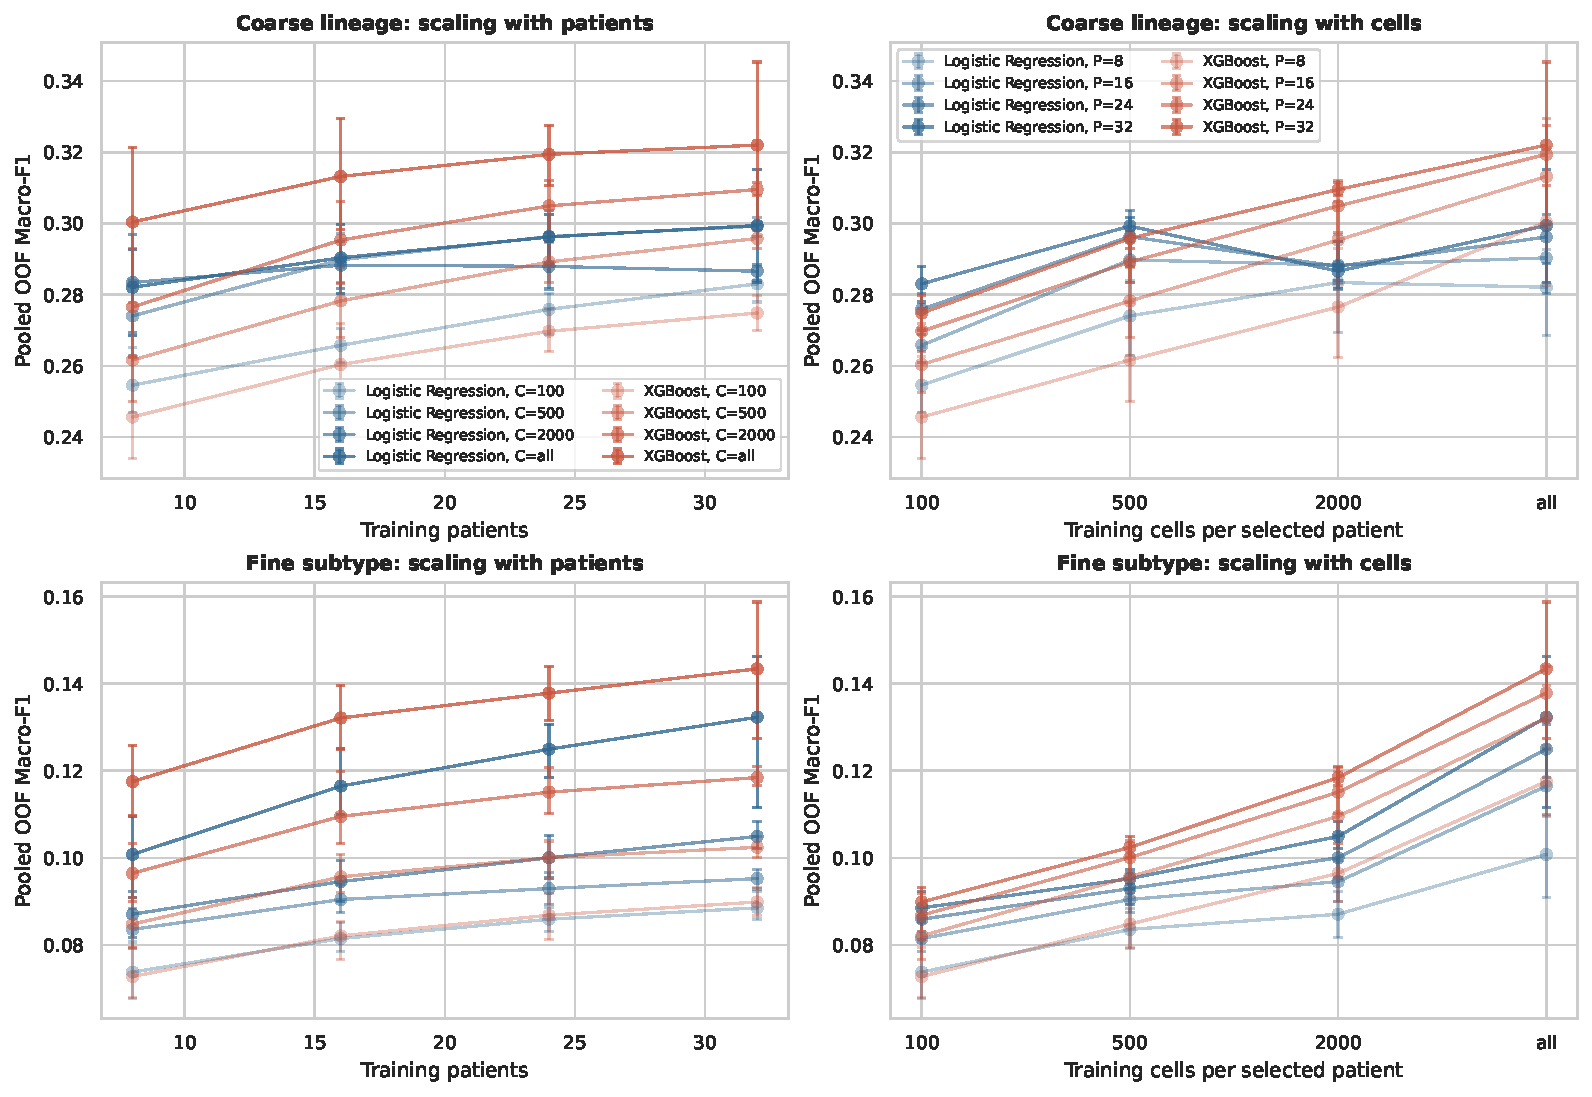
\includegraphics[width=\textwidth]{figures/patient_scaling_curves.pdf}
\caption{Patient-budget curves at each fixed per-patient cell cap. Intervals
show subset-resampling variability; they do not represent uncertainty over a
new patient population. Non-monotonic local changes are retained rather than
smoothed.}
\label{fig:patient_scaling_curves}
\end{figure}

The surface is cohort- and range-specific. We do not compare its unequal
endpoints or use it to establish a patient- or cell-dominant scaling law, and it
cannot estimate the benefit of patients drawn from new sites or acquisition
batches.

\bibliography{iclr2027_conference}
\bibliographystyle{iclr2027_conference}
\end{document}
